\section{Introduction}
Step counting from commodity smartphone sensors is a practical yet non-trivial time-series problem because sensor orientation, attachment location, gait variability, and sampling conditions can change substantially between users and sessions. This project develops a unified end-to-end pipeline for inertial measurement unit (IMU) based step counting, with one consistent interface that supports both offline batch processing and online streaming updates.

The system is implemented around a causal neural temporal model that predicts both frame-level step events and window-level step counts. The same model and post-processing logic are used in evaluation scripts and real-time demos, which improves consistency between training objectives and deployment behavior.

From an academic perspective, the core practical contributions are summarized in Table~\ref{tab:intro_contributions}. The results show strong performance on personal recordings and highlight remaining generalization gaps in cross-participant and wrist-mounted settings.

\begin{table}[H]
\centering
\caption{Core practical contributions of this work.}
\label{tab:intro_contributions}
\small
\begin{tabular}{p{0.20\linewidth}p{0.68\linewidth}}
\toprule
Contribution & Description \\
\midrule
Reproducible workflow & End-to-end data-to-inference pipeline for smartphone accelerometer signals. \\
Causal streaming design & Causal inference architecture and logic suitable for low-latency online updates. \\
Empirical analysis & Evaluation across public benchmark-style data and self-recorded sessions. \\
\bottomrule
\end{tabular}
\end{table}

\section{Data Collection}
\subsection{Datasets and Sources}
Two data sources are used in this study. The first is a publicly available dataset with four modalities (hip and wrist at 100~Hz and 25~Hz)~\cite{oxwalk}. The second consists of self-recorded sessions collected with a smartphone application for real-time sensing and remote polling~\cite{phyphox}.

The first source provides controlled multi-participant recordings and is primarily used for model development and quantitative benchmarking. The second source captures realistic personal usage conditions and is used to evaluate practical deployment behavior, including end-to-end counting accuracy under naturally occurring motion variations.

\subsection{Preprocessing}
Raw records are processed by a deterministic pipeline prior to model inference. Each sequence is sorted by timestamp, duplicate timestamps are removed, and tri-axial acceleration is resampled to 50~Hz through linear interpolation. This resampling step standardizes heterogeneous acquisition rates and enables a single model configuration across all evaluation settings.

Let the irregularly sampled acceleration sequence be $\{(t_i, \mathbf{a}_i)\}_{i=1}^{N}$ where $\mathbf{a}_i=[a_x,a_y,a_z]^\top$. A uniform grid $\{\tau_k\}$ at 50~Hz is constructed, and each axis is interpolated independently to obtain $\tilde{\mathbf{a}}(\tau_k)$. In addition, acceleration magnitude is computed as
\begin{equation}
a_{mag}(t)=\sqrt{a_x(t)^2+a_y(t)^2+a_z(t)^2},
\end{equation}
which serves as a robust orientation-insensitive feature for downstream temporal modeling.

\section{Algorithm}
\subsection{Problem Formulation}
Given a multivariate acceleration sequence $\mathbf{X}=\{\mathbf{x}_t\}_{t=1}^{T}$, the objective is to estimate both (i) step-event likelihoods at each frame and (ii) cumulative step count over a time interval. Formally, the model outputs
\begin{equation}
\hat{p}_t = P(\text{step at } t\mid \mathbf{X}_{\le t}), \qquad
\hat{c}_{w}=f_c(\mathbf{X}_{w}),
\end{equation}
where $\hat{p}_t$ is causal and $\hat{c}_{w}$ is the predicted count for window $w$.

This dual-head setup encourages local event sensitivity and global counting stability simultaneously. In practice, frame-level probabilities are converted into discrete events via thresholding and local-maximum detection with refractory constraints.

\subsection{Model and Features}
The model is defined as a causal temporal network (TCN) with residual dilated 1D convolutions and two prediction heads~\cite{bai2018tcn}. The event head produces per-frame step-event logits, while the count head performs window-level step-count regression.

Input features are four-dimensional per sample:
\begin{equation}
\begin{aligned}
\mathbf{x}_t &= [a_x(t), a_y(t), a_z(t), a_{mag}(t)], \\
a_{mag}(t) &= \sqrt{a_x(t)^2+a_y(t)^2+a_z(t)^2}.
\end{aligned}
\end{equation}

The causal architecture ensures that predictions at time $t$ depend only on past and current context, which is critical for real-time usage. Dilated convolutions increase receptive field length without requiring recurrent state, enabling efficient inference on streaming chunks.

\subsection{Training Pipeline}
Training involves participant-level split construction with the key settings summarized in Table~\ref{tab:train_settings}.

\begin{table}[H]
\centering
\caption{Core training configuration.}
\label{tab:train_settings}
\small
\begin{tabular}{ll}
\toprule
Setting & Value \\
\midrule
Sample rate & 50~Hz \\
Window length / stride & 4.0~s / 0.5~s \\
Label smoothing & Gaussian kernel, $\sigma=0.06$~s \\
Loss & BCEWithLogits + weighted MSE \\
Optimizer & AdamW with early stopping \\
\bottomrule
\end{tabular}
\end{table}

Label smoothing in the event target is implemented with a Gaussian kernel, which softens annotation noise near heel-strike timing and empirically stabilizes optimization. The total objective combines event classification and count regression:
\begin{equation}
\mathcal{L}=\mathcal{L}_{event}+\lambda\,\mathcal{L}_{count},
\end{equation}
where $\mathcal{L}_{event}$ is binary cross-entropy on frame labels and $\mathcal{L}_{count}$ is weighted mean squared error on window-level counts.

Early stopping is selected based on validation loss to reduce overfitting and preserve generalization. The released checkpoint and accompanying metrics indicate that this protocol yields a robust baseline for both offline and streaming inference.

\subsection{Online/Offline Inference Logic}
The system wraps the neural model and exposes the required API for resetting, updating, and running offline inference. Streaming inference maintains a context buffer and converts event probabilities to step timestamps using local-maximum detection with threshold and refractory constraints. The operational inference parameters are summarized in Table~\ref{tab:infer_params}.

\begin{table}[H]
\centering
\caption{Streaming inference parameters.}
\label{tab:infer_params}
\small
\begin{tabular}{ll}
\toprule
Parameter & Value \\
\midrule
Probability threshold & $p_{th}=0.68$ \\
Minimum inter-step interval & 0.33~s \\
Context length & 4.0~s \\
\bottomrule
\end{tabular}
\end{table}

The online update routine processes only newly arrived samples and appends them to a fixed-length context. A new step is emitted when a local maximum exceeds the probability threshold and the time since the previous accepted step is greater than the minimum inter-step interval. This mechanism suppresses bursty false positives while retaining responsiveness to cadence changes.

Offline processing uses the same post-processing logic to avoid train-test and offline-online mismatches. This design choice also simplifies interpretability: threshold and refractory parameters have a consistent meaning in all execution modes.

\section{Results}
\subsection{Evaluation Protocol}
Evaluation levels are summarized in Table~\ref{tab:eval_levels}. Absolute error and relative error are emphasized because they directly reflect practical counting quality.

\begin{table}[H]
\centering
\caption{Evaluation levels used in this study.}
\label{tab:eval_levels}
\small
\begin{tabular}{p{0.20\linewidth}p{0.68\linewidth}}
\toprule
Level & Description \\
\midrule
Neural model metrics & Participant-level split evaluation of event and count prediction quality. \\
End-to-end personal sessions & Full counting performance on two self-recorded sessions. \\
Deterministic subset calibration & Stress-test style evaluation on challenging cross-domain subset examples. \\
\bottomrule
\end{tabular}
\end{table}

\subsection{Model Metrics}
The temporal model metrics on validation and test splits are listed in Table~\ref{tab:model_metrics}.

\begin{table}[H]
\centering
\caption{Neural model performance metrics.}
\label{tab:model_metrics}
\small
\begin{tabular}{lr}
\toprule
Metric & Value \\
\midrule
Best validation loss & 0.3732 \\
Test event loss & 0.3364 \\
Test count MAE (window-level) & 0.4840 \\
\bottomrule
\end{tabular}
\end{table}

These values indicate that the event head learns reliable frame-level structure while the count head remains accurate at window scale. The low test count MAE supports using count-aware supervision in addition to event supervision.

\subsection{Inference on Self-Recorded Sessions}
Inference on self-recorded sessions demonstrates low counting error in realistic user conditions:
\begin{table}[H]
\centering
\caption{Inference results on two self-recorded sessions.}
\label{tab:self_results}
\small
\begin{tabular}{lrrrr}
\toprule
Session & GT & Est. & Abs. err. & Rel. err. (\%) \\
\midrule
Session 1 & 84 & 82 & 2 & 2.38 \\
Session 2 & 100 & 101 & 1 & 1.00 \\
\bottomrule
\end{tabular}
\end{table}

Across both sessions, mean absolute error is 1.5 steps and mean absolute percentage error is 1.69\%, indicating high practical reliability for the tested personal recordings.

\begin{figure}[H]
\centering
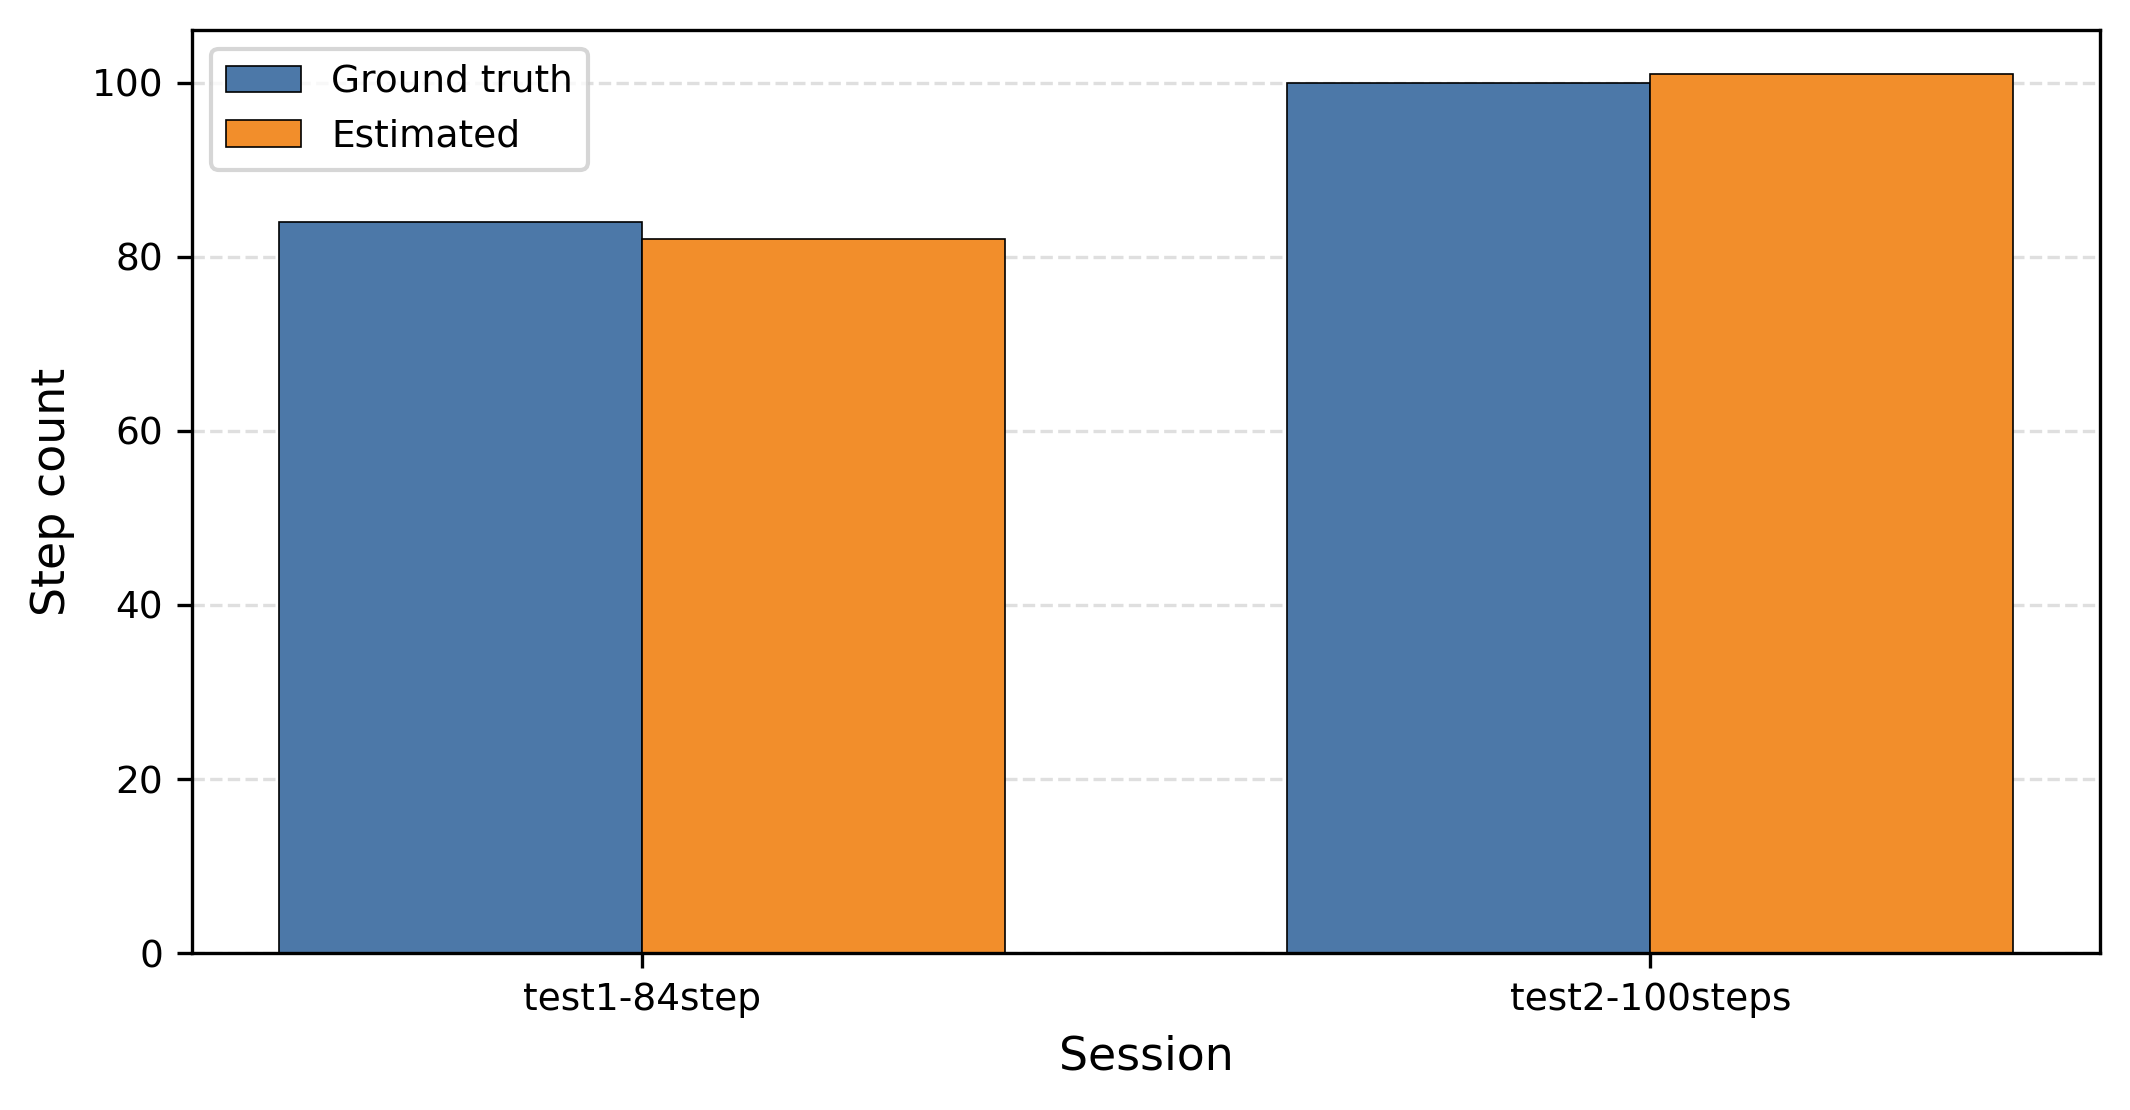
\includegraphics[width=\linewidth]{fig/self_sessions_gt_vs_est.png}
\caption{Ground-truth versus estimated step counts on self-recorded sessions.}
\label{fig:self_gt_est}
\end{figure}

\subsection{Subset Calibration/Evaluation}
A deterministic subset evaluation yields MAE $=15.6$ steps and MAPE $=17.51\%$.

Compared with the personal-session results, this gap suggests that cross-participant and wrist scenarios remain the dominant challenge. To characterize this behavior, per-sample absolute errors are visualized in Fig.~\ref{fig:subset_abs_error}.

\begin{figure}[H]
\centering
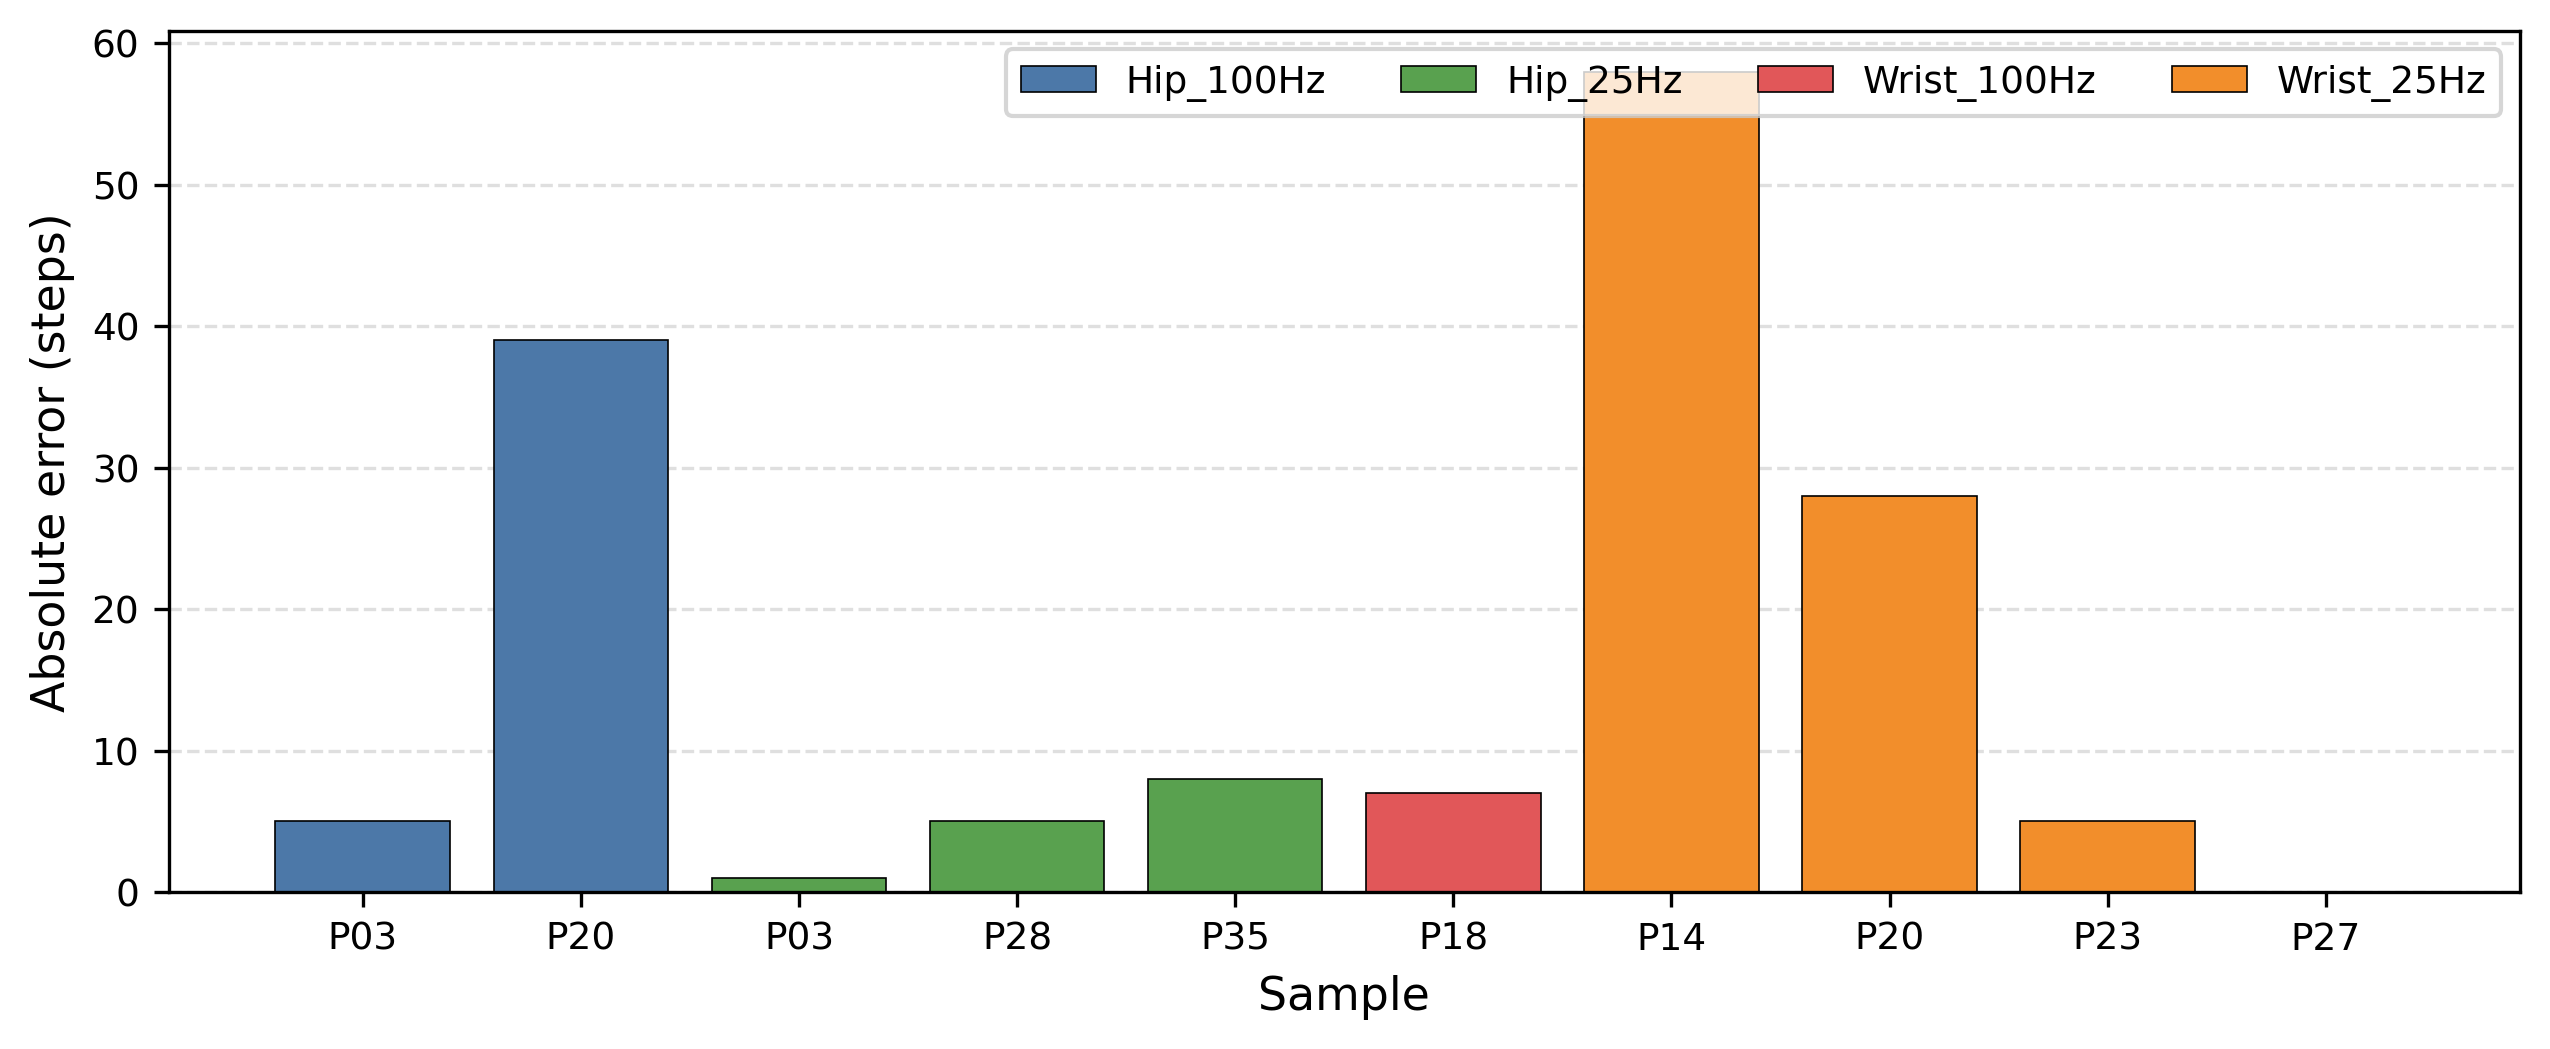
\includegraphics[width=\linewidth]{fig/calibration_subset_abs_error.png}
\caption{Absolute error distribution on the deterministic subset evaluation. Colors indicate sensor placement and sampling modality.}
\label{fig:subset_abs_error}
\end{figure}

\begin{table}[H]
\centering
\caption{Modality-level absolute error summary on the deterministic subset.}
\label{tab:modality_abs_error}
\small
\begin{tabular}{lrr}
\toprule
Modality & Samples & Mean abs. error (steps) \\
\midrule
Hip 100~Hz & 2 & 22.00 \\
Hip 25~Hz & 3 & 4.67 \\
Wrist 100~Hz & 1 & 7.00 \\
Wrist 25~Hz & 4 & 22.75 \\
\bottomrule
\end{tabular}
\end{table}

The modality breakdown indicates that wrist 25~Hz and hip 100~Hz examples contribute most of the error mass in this subset, while hip 25~Hz remains comparatively stable. This pattern is consistent with known sensitivity of step-event signatures to placement and motion style.

\section{Real-Time Demo}
Two real-time demos are implemented: a Matplotlib-based live visualization with cumulative counts, and a browser-based dashboard with live traces and step markers.

\begin{figure}[H]
\centering
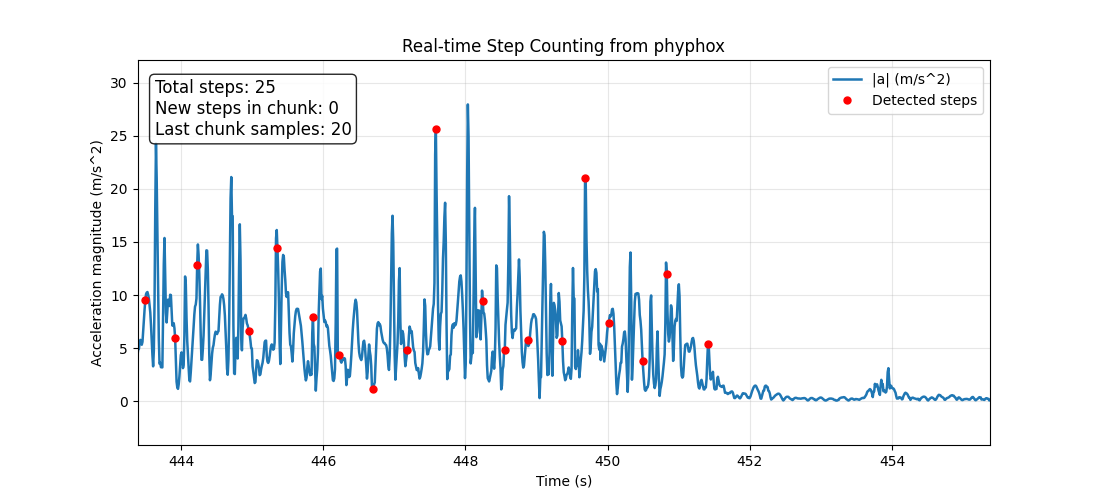
\includegraphics[width=\linewidth]{fig/counterpython.png}
\caption{Matplotlib-based real-time demo showing live acceleration traces and cumulative step count.}
\label{fig:counter_python}
\end{figure}


\begin{figure}[H]
\centering
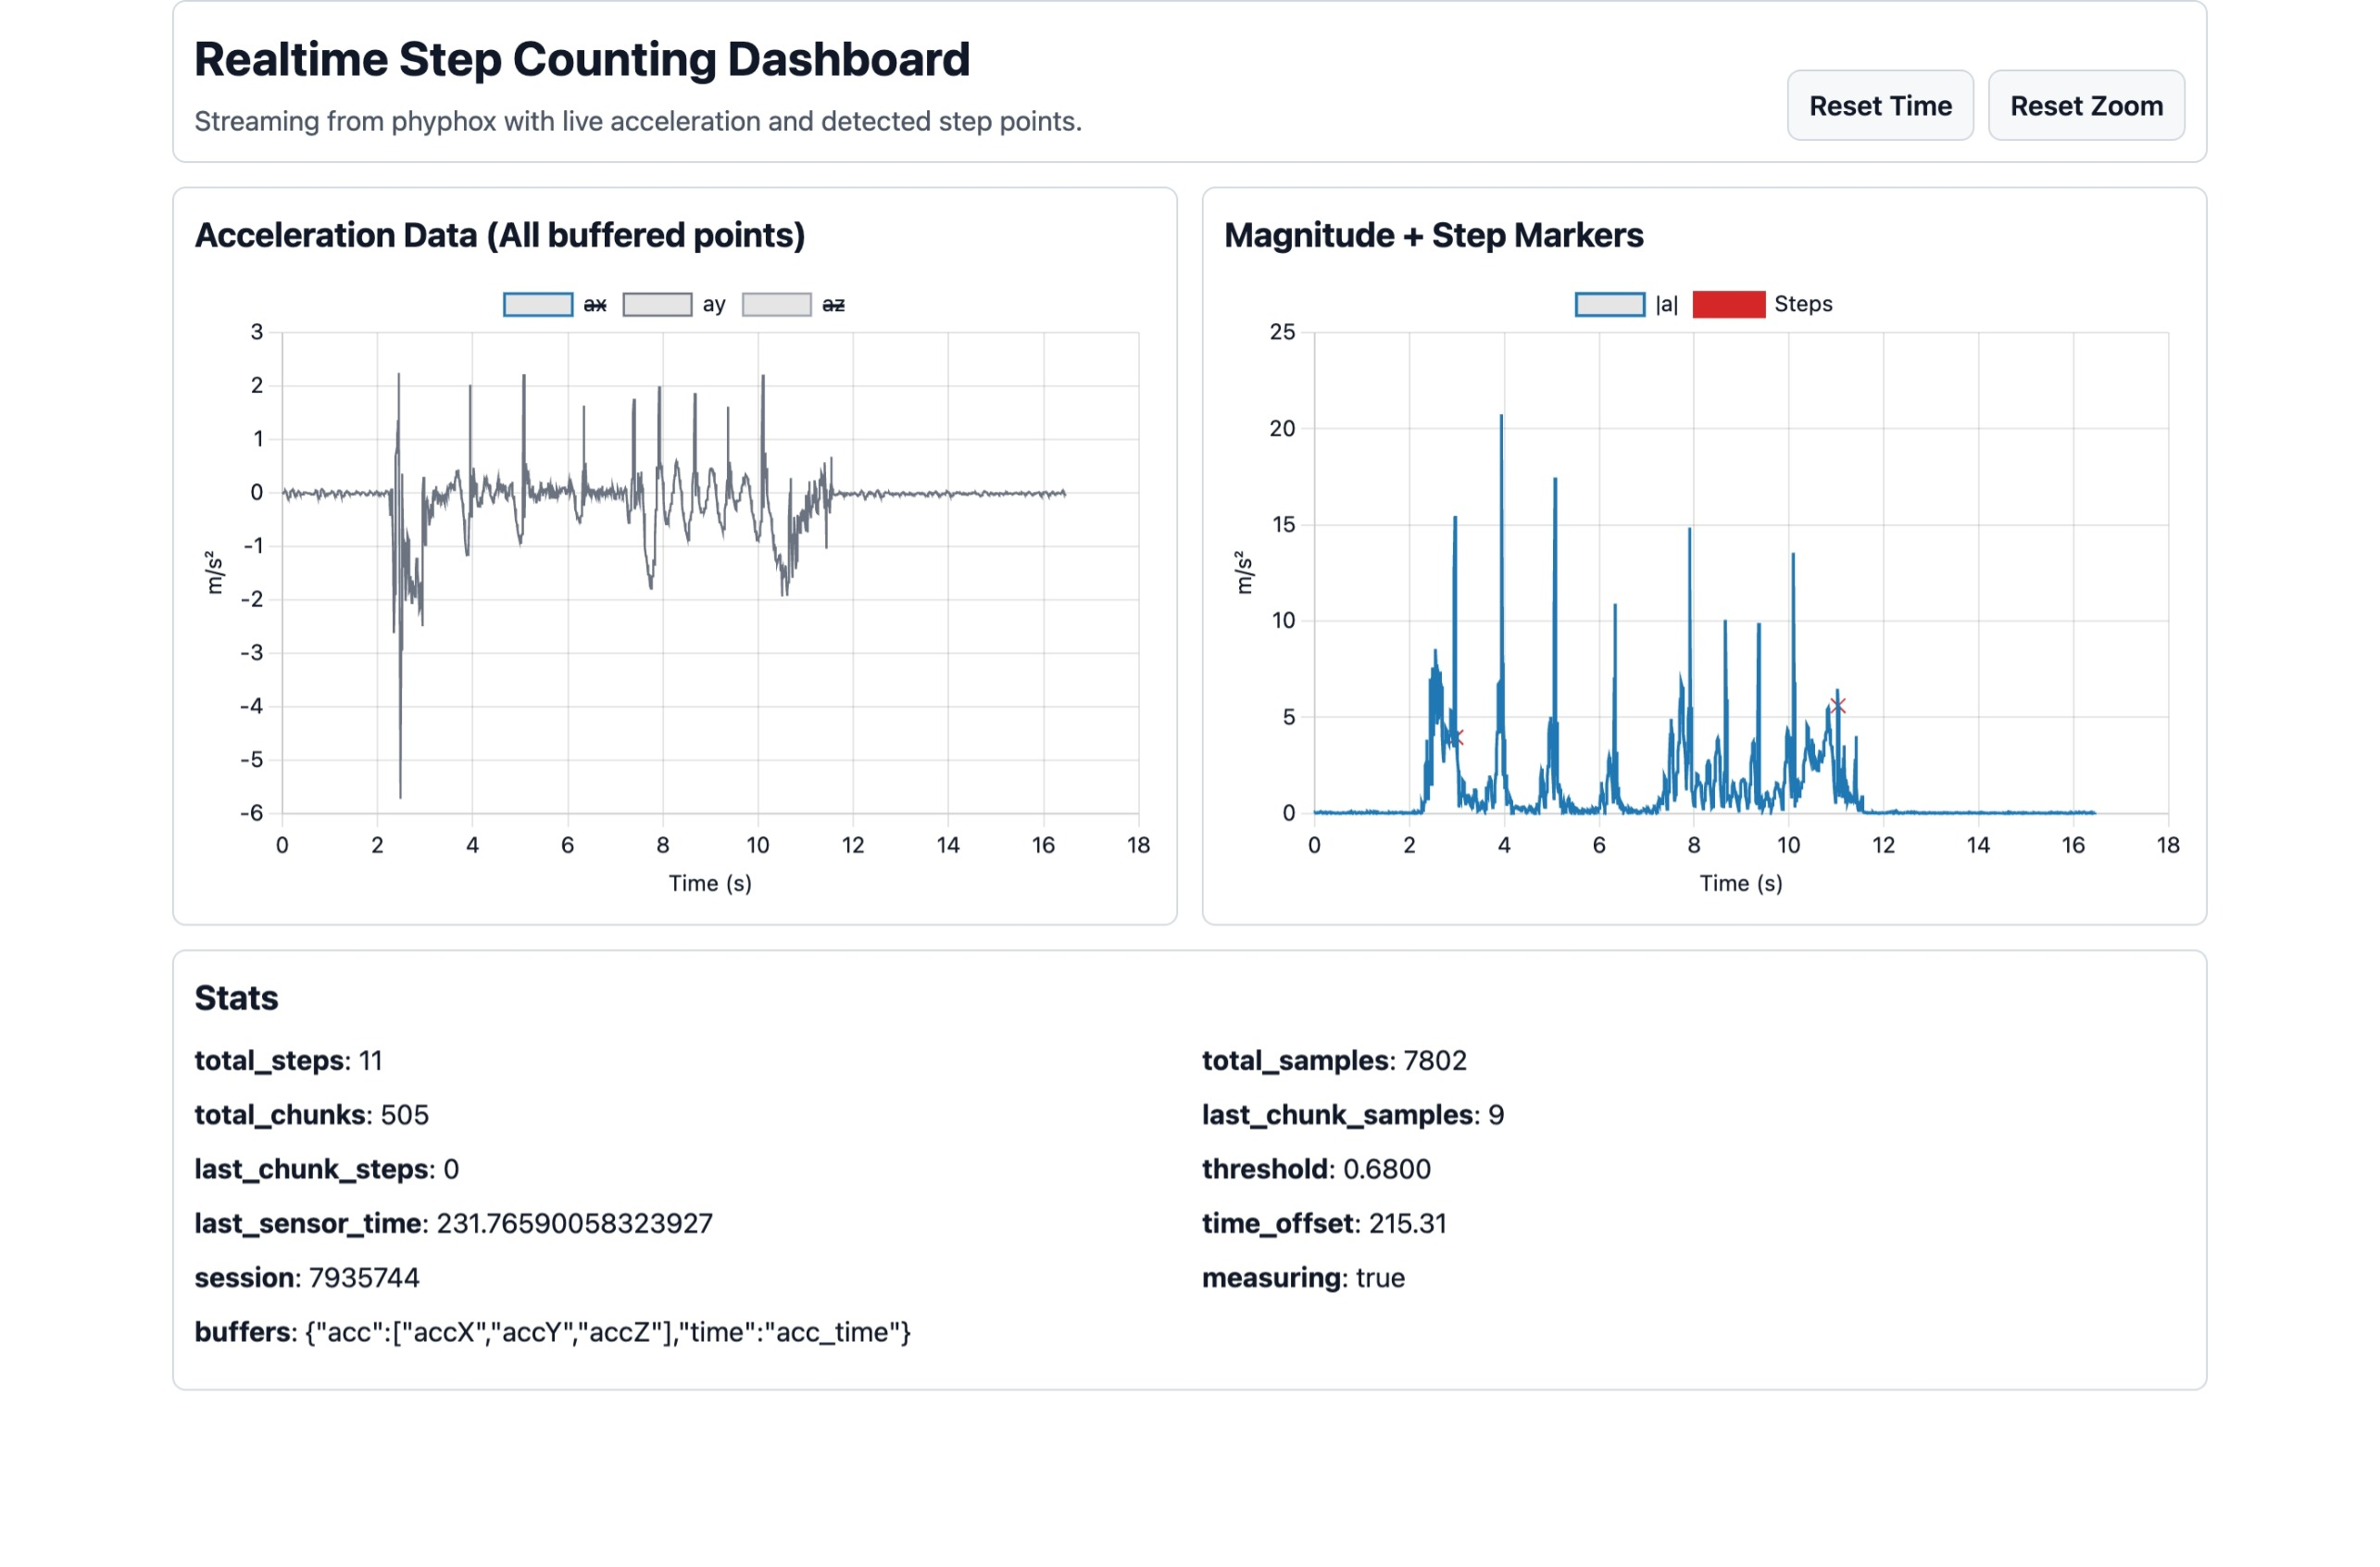
\includegraphics[width=\linewidth]{fig/realtimeweb.jpeg}
\caption{Browser-based real-time demo showing live acceleration traces and detected step events.}
\label{fig:realtime_web}
\end{figure}

Both demos process only newly arrived samples and support session reset handling.

\subsection{Operational Characteristics}
The real-time pipeline emphasizes low latency and predictable update behavior. Because inference is causal and chunk-based, the system avoids look-ahead dependencies and can operate continuously under streaming sensor input. In addition, session reset handling prevents stale state carry-over between recording intervals, which is important in practical classroom or field demonstrations.

\subsection{Example Signal-Level Outputs}
Representative signal-level visualizations from two test cases are shown below.

\begin{figure}[H]
\centering
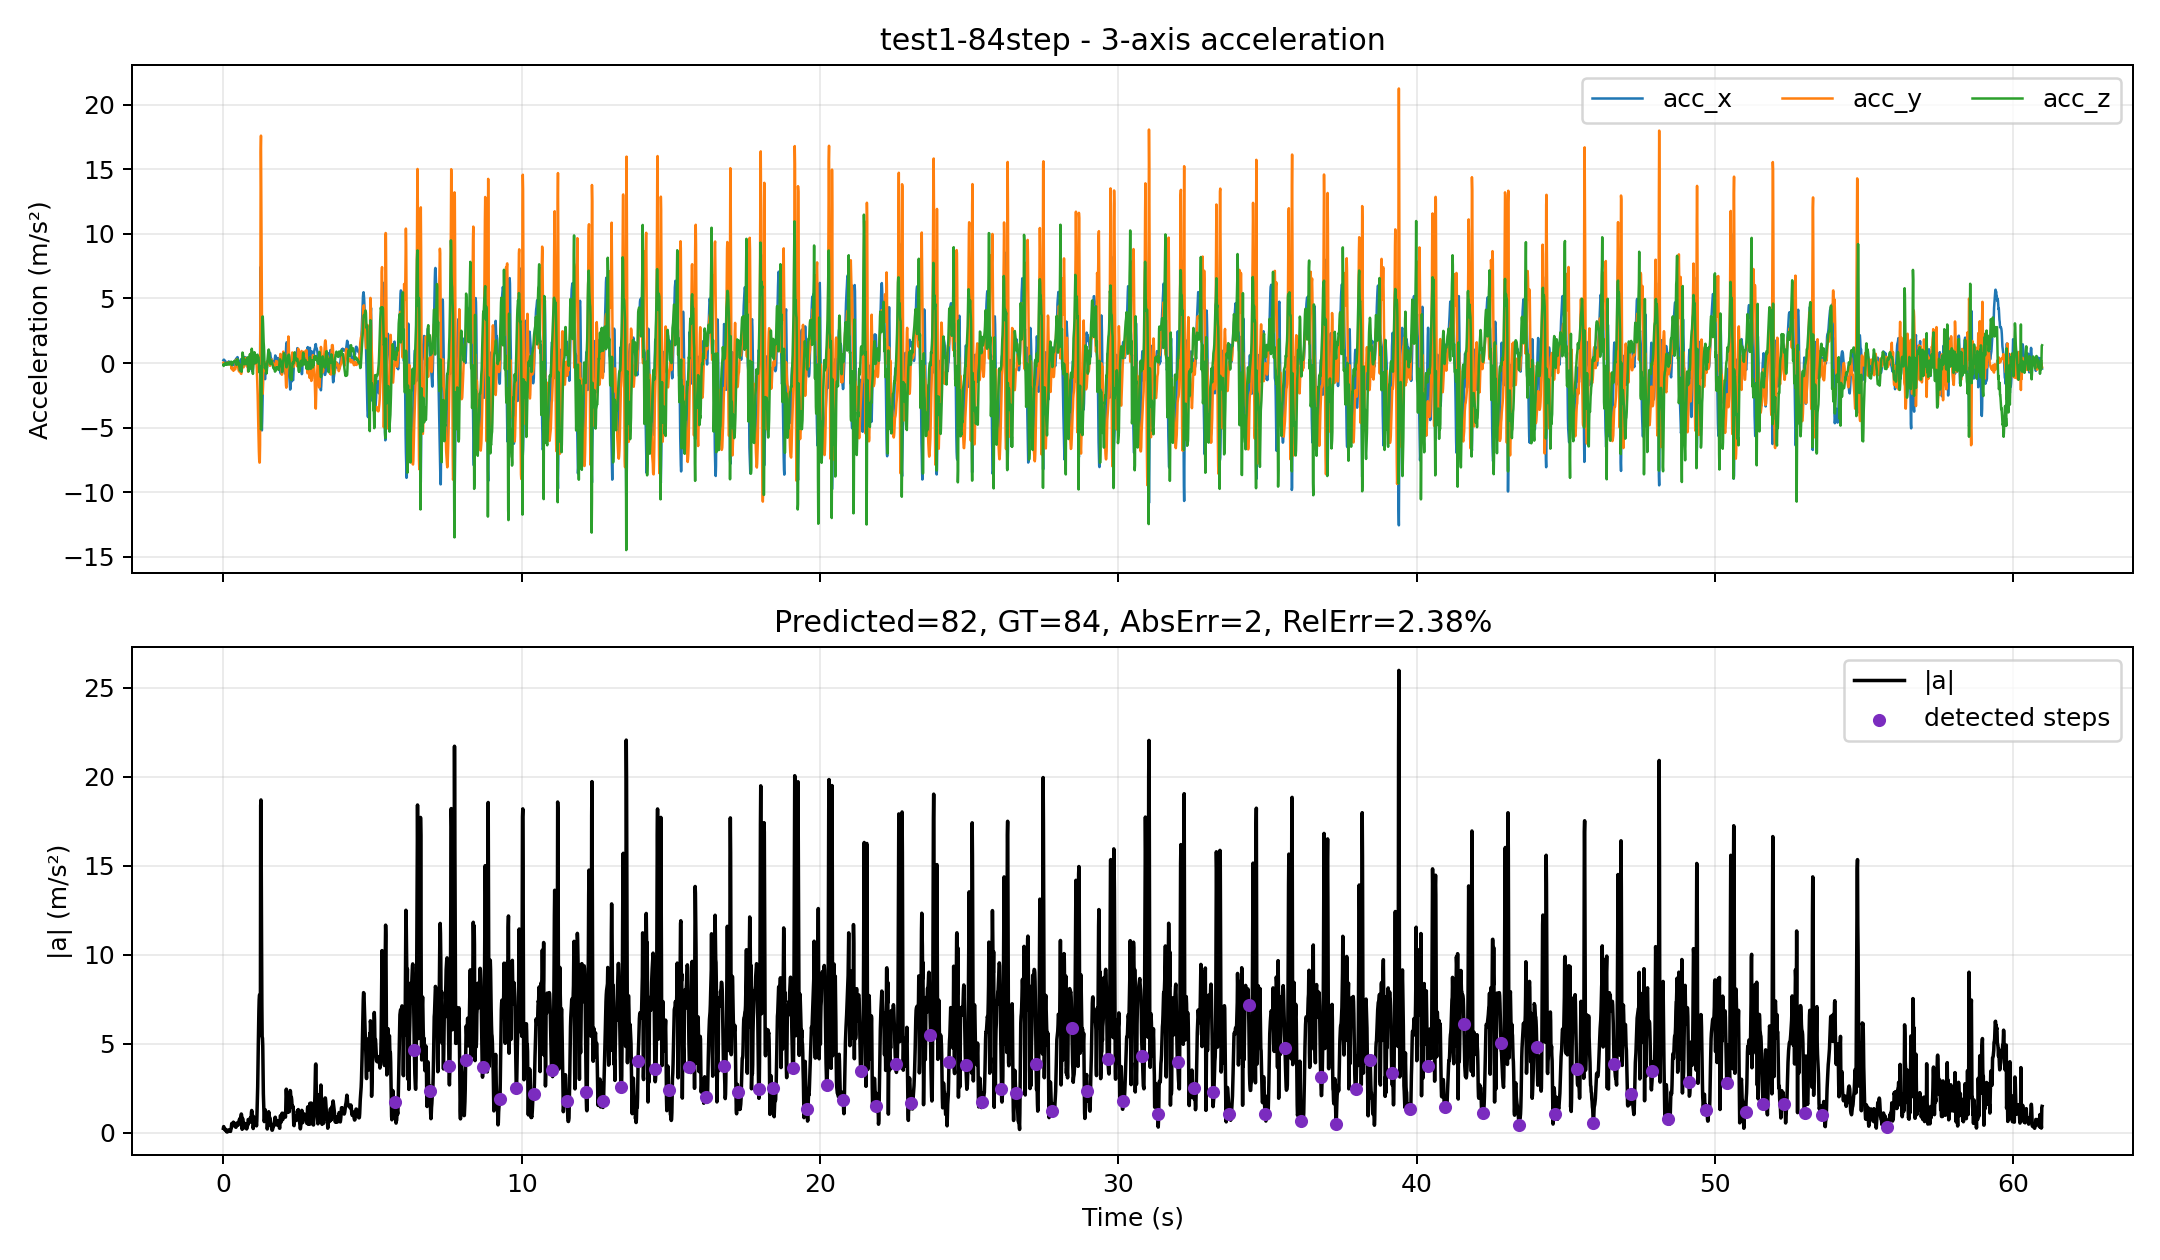
\includegraphics[width=\linewidth]{fig/test1-84step_plot.png}
\caption{Test case 1: three-axis acceleration (top) and magnitude with detected step timestamps (bottom).}
\label{fig:test1_plot}
\end{figure}

\begin{figure}[H]
\centering
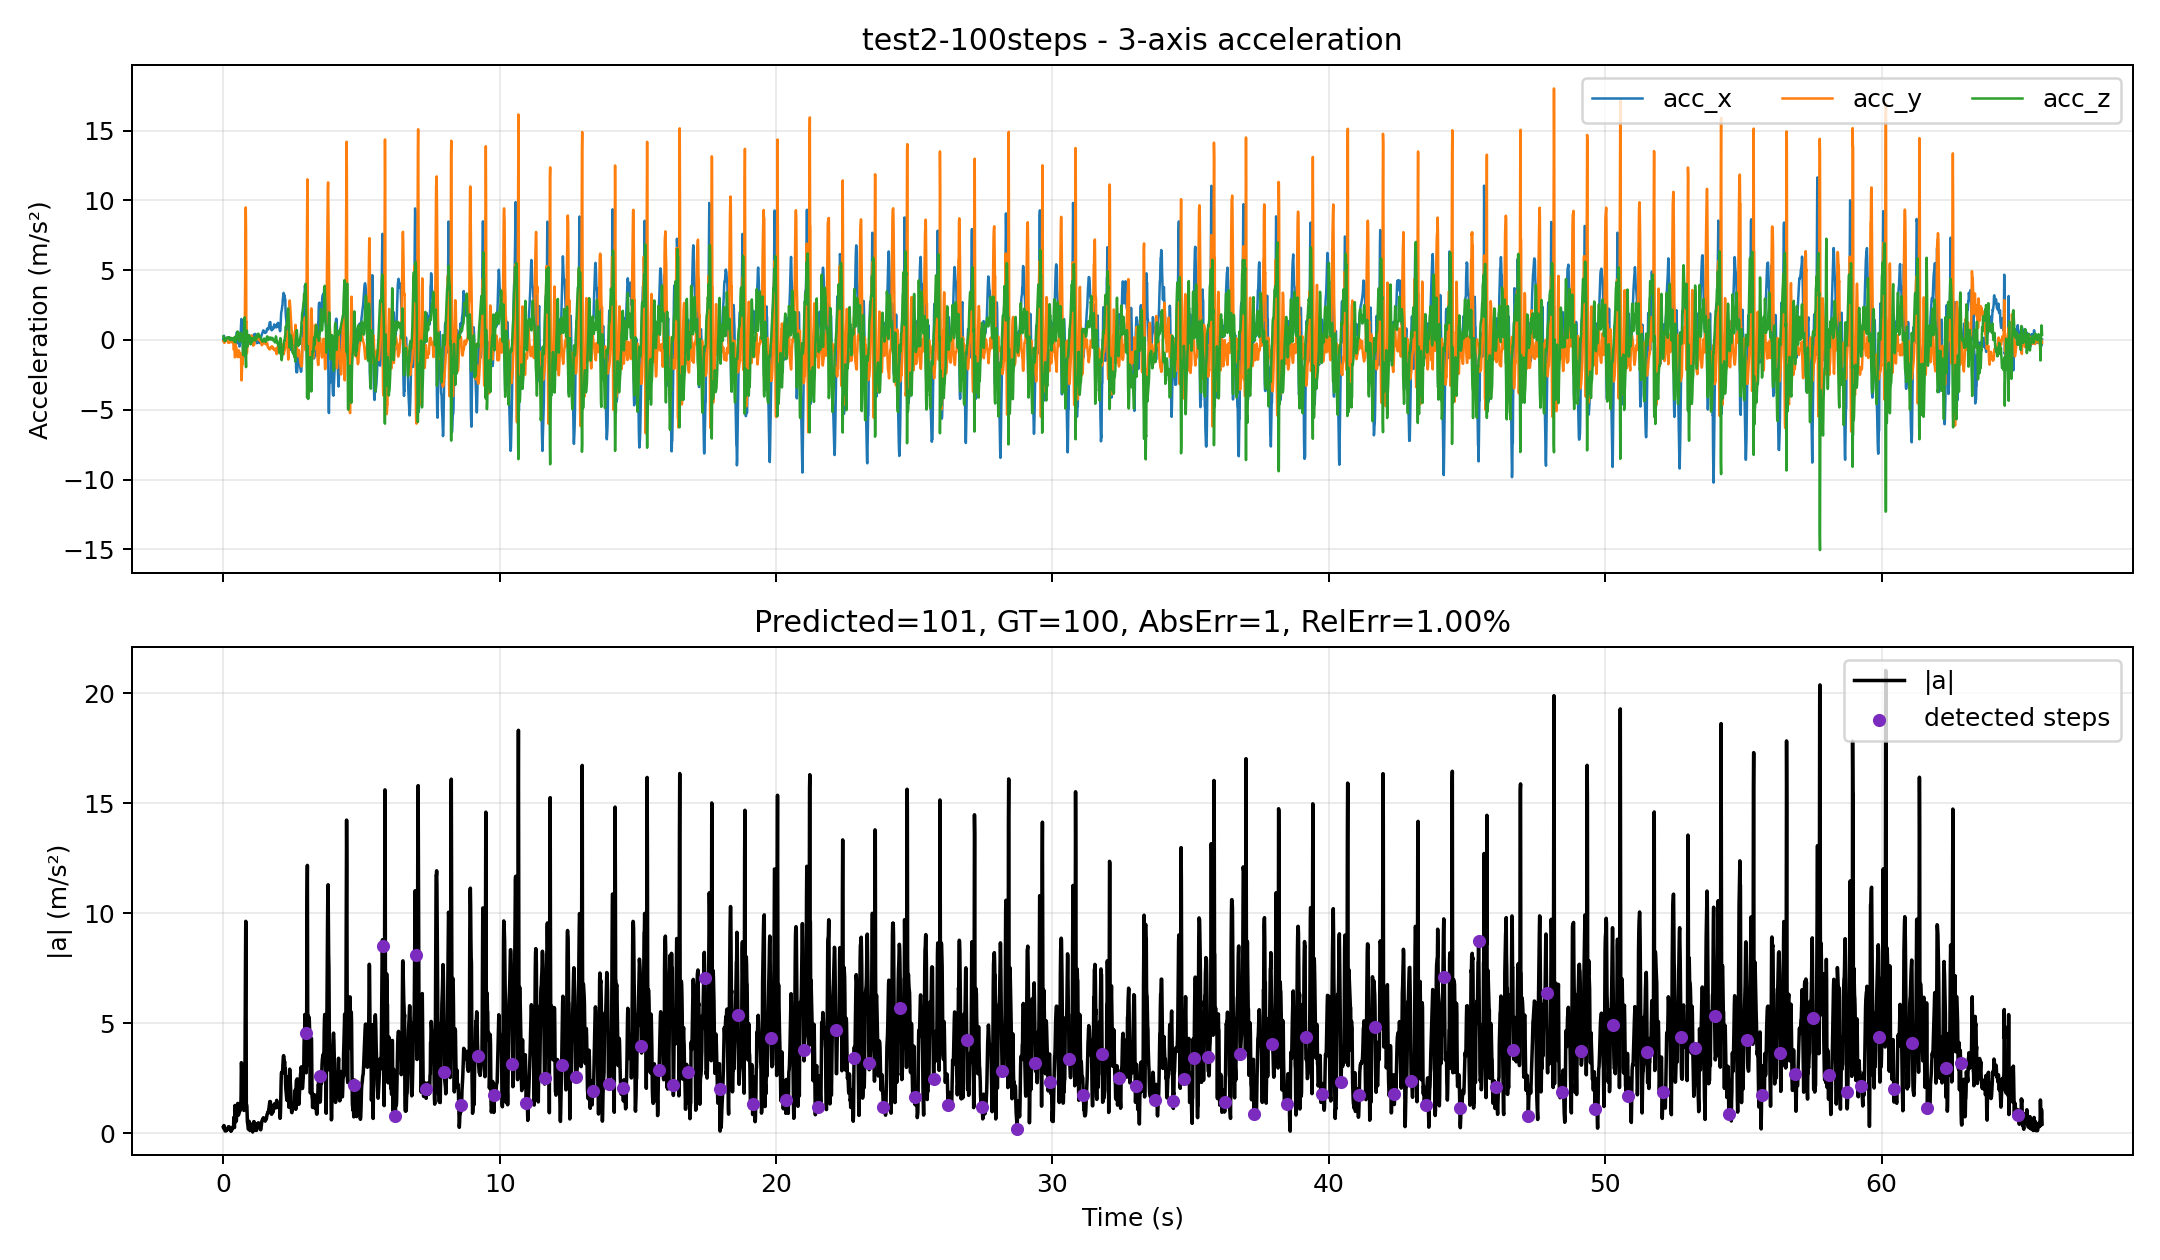
\includegraphics[width=\linewidth]{fig/test2-100steps_plot.png}
\caption{Test case 2: three-axis acceleration (top) and magnitude with detected step timestamps (bottom).}
\label{fig:test2_plot}
\end{figure}

In both examples, detected events align well with oscillatory peaks in acceleration magnitude. Minor discrepancies typically occur near transition segments (start/stop motion), where cadence regularity is lower and false peak rejection becomes more difficult.

\section{Discussion}
\subsection{Strengths}
The system provides a unified API for offline grading and real-time deployment, and its causal chunk-wise update strategy is well suited for streaming operation. It also demonstrates good accuracy on personal test recordings and offers a reproducible inference and visualization workflow that supports transparent analysis.

\subsection{Limitations}
Generalization gaps remain across participants and placement modalities, especially in wrist scenarios with irregular arm motion. In addition, the current threshold/refractory post-processing is globally fixed and may not be optimal for all gait regimes. Evaluation of edge cases, such as abrupt turns, phone handling changes, and non-walking periodic motion, is also still limited.

\subsection{Threats to Validity}
Threats to validity are summarized in Table~\ref{tab:validity_threats}.

\begin{table}[H]
\centering
\caption{Key threats to validity.}
\label{tab:validity_threats}
\small
\begin{tabular}{p{0.20\linewidth}p{0.68\linewidth}}
\toprule
Threat & Description \\
\midrule
Limited personal-session count & Personal-session evaluation includes only two recordings and may overestimate robustness. \\
Limited calibration subset size & Deterministic subset calibration uses few samples and is better interpreted as stress testing than comprehensive benchmarking. \\
Ground-truth uncertainty & Free-living annotation uncertainty can affect event-level alignment even when aggregate counts remain accurate. \\
\bottomrule
\end{tabular}
\end{table}

\subsection{Future Work}
Future improvements include domain adaptation for placement shifts, uncertainty-aware decision thresholds, and lightweight personalization from short calibration walks. Additional ablations on context length, threshold settings, and sampling-rate robustness would further clarify performance trade-offs for deployment.

\section{Conclusion}
This work presents an end-to-end smartphone IMU step-counting system that unifies offline processing and real-time streaming under a single causal neural framework. The model delivers strong counting accuracy on personal recordings and demonstrates practical deployability through live demos. At the same time, subset-level analysis reveals meaningful cross-domain challenges, especially for certain wrist and participant conditions. Overall, the implementation provides a strong reproducible baseline and a clear path toward improved robustness through modality-aware adaptation and personalization.
